\documentclass[11pt]{article}

\usepackage[T1]{fontenc}
\usepackage[utf8]{inputenc}
\usepackage{lmodern}
\usepackage{microtype}
\usepackage[a4paper,margin=22mm,headheight=15pt]{geometry}
\usepackage{amsmath,amssymb,bm,mathtools}
\usepackage{booktabs,tabularx,array,multirow}
\usepackage{siunitx}
\usepackage{graphicx}
\usepackage{xcolor}
\usepackage{tikz}
\usetikzlibrary{arrows.meta,positioning,fit,calc}
\usepackage{caption}
\usepackage{subcaption}
\usepackage{enumitem}
\usepackage{parskip}
\usepackage{fancyhdr}
\usepackage{hyperref}
\usepackage{etoolbox}
\usepackage[nameinlink,capitalise]{cleveref}

\definecolor{negfblue}{HTML}{0072B2}
\definecolor{negforange}{HTML}{D55E00}
\definecolor{negfgreen}{HTML}{009E73}
\definecolor{negfgray}{HTML}{666666}
\definecolor{statusbg}{HTML}{EEF5F9}
\definecolor{warningbg}{HTML}{FFF4E6}

\hypersetup{
  colorlinks=true,
  linkcolor=negfblue,
  citecolor=negfgreen,
  urlcolor=negfblue,
  pdftitle={NEGFPy phonon-phonon NEGF toy-model validation},
  pdfauthor={NEGFPy project},
  pdfsubject={Anharmonic phonon transport formulation and benchmarks}
}

\sisetup{
  scientific-notation=true,
  round-mode=places,
  round-precision=3,
  detect-all=true
}

\IfFileExists{release_config.tex}{%
  \input{release_config.tex}%
}{%
  \PackageError{NEGFPy toy-gate report}
    {Missing required release_config.tex}
    {Generate release_config.tex from the verified scaling and release
     runner artifacts before compiling this report.}%
  \stop
}
\newcommand{\RequireReleaseConfigMacro}[1]{%
  \ifcsdef{#1}{}{%
    \PackageError{NEGFPy toy-gate report}
      {Required release configuration macro #1 is missing}
      {Regenerate release_config.tex from verified artifacts.}%
    \stop
  }%
}
\forcsvlist{\RequireReleaseConfigMacro}{%
  ProductionStagingDir,ProductionFigureDir,HistoricalFigureDir,%
  ExpectedToyGateCommit,ReportDate,MPIRankLadder,MPIFastestRankCount,%
  MPICandidateRankCount,MPIReleaseRankCount,MPISiliconRankCount,MPIReleaseMode,%
  MPIBaselineWallSeconds,MPICandidateWallSeconds,MPICandidateSpeedup,%
  MPIMaxMemoryFractionObserved,MPISocketCount,MPIScalingPhysicsSHA,%
  MPIReleasePhysicsSHA,MPIScalingManifestSHA,MPIRunnerManifestSHA,%
  MPIExecutionManifestSHA,CurrentAttemptSHA,AttemptPublicationSHA,%
  MPIReleaseLaunchIntentSHA,MPIReleaseLaunchIntentPayloadSHA,%
  MPIReleaseLaunchSHA,MPIReleaseLaunchPayloadSHA,%
  MPIExecutionSourceIdentitySHA,MPIEnvironmentPrefixManifestSHA,%
  MPILaunchEnvironmentSHA,%
  ArtifactSHA256SUMSRawSHA,ArtifactFetchReceiptSHA,%
  StagingSHA256SUMSRawSHA,StagingImportReceiptSHA,%
  ProductionFiguresSHA256SUMSRawSHA,ProductionFiguresReceiptSHA,%
  HistoricalFiguresSHA256SUMSRawSHA,HistoricalFiguresReceiptSHA,%
  ReleaseStrictReportFileSHA,ReleaseStrictReportBodySHA,%
  MPIToyMinimumSpeedupSatisfied,MPIScalingPassed,MPIPhysicsEqualityPassed,%
  MPIBindingPassed,MPIMemoryPreflightPassed,MPIRunnerReleaseCertified}
\newcommand{\RequireReleaseConfigTrue}[2]{%
  \ifdefstring{#1}{true}{}{%
    \PackageError{NEGFPy toy-gate report}
      {Release configuration gate #2 is not true (#1)}
      {Regenerate release_config.tex from verified remote artifacts.}%
    \stop
  }%
}
\RequireReleaseConfigTrue{\MPIScalingPassed}{MPI scaling ladder}
\RequireReleaseConfigTrue{\MPIPhysicsEqualityPassed}{MPI physics equality}
\RequireReleaseConfigTrue{\MPIBindingPassed}{MPI binding}
\RequireReleaseConfigTrue{\MPIMemoryPreflightPassed}{MPI memory preflight}
\RequireReleaseConfigTrue{\MPIRunnerReleaseCertified}{MPI release runner}
\def\ToyGateReleaseCertified{missing}
\def\ToyGateOraclePassed{missing}
\def\ToyGateMultidimensionalPassed{missing}
\def\ToyGateStaticConfigurationPassed{missing}
\def\ToyGateRuntimeEvidencePassed{missing}
\def\ToyGateCommit{missing}
\def\ToyGateWeakCouplingCoverage{missing}
\def\ToyGateWeakCouplingPassed{missing}
\def\ToyGateWeakCouplingMaxLinewidthRatio{missing}
\def\ToyGateWeakCouplingMaxShiftRatio{missing}
\def\ToyGateWeakCouplingLimit{missing}
\def\ToyGateMultidimensionalWeakCouplingCoverage{missing}
\def\ToyGateMultidimensionalWeakCouplingPassed{missing}
\def\ToyGateMultidimensionalWeakCouplingMaxLinewidthRatio{missing}
\def\ToyGateMultidimensionalWeakCouplingMaxShiftRatio{missing}
\def\ToyGateMultidimensionalWeakCouplingLimit{missing}
\IfFileExists{\ProductionStagingDir/tex/release_summary.tex}{%
  \input{\ProductionStagingDir/tex/release_summary.tex}%
}{%
  \PackageError{NEGFPy toy-gate report}
    {Missing certified production staging file
     \ProductionStagingDir/tex/release_summary.tex}
    {Import and verify the immutable production campaign before compiling
     this report. Provisional or legacy benchmark data are not accepted.}%
  \stop
}
\IfFileExists{\ProductionStagingDir/tex/weak_coupling_summary.tex}{%
  \input{\ProductionStagingDir/tex/weak_coupling_summary.tex}%
}{%
  \PackageError{NEGFPy toy-gate report}
    {Missing imported weak-coupling summary}
    {Import the complete strict campaign before compiling this report.}%
  \stop
}
\IfFileExists{\ProductionStagingDir/tex/multidimensional_weak_coupling_summary.tex}{%
  \input{\ProductionStagingDir/tex/multidimensional_weak_coupling_summary.tex}%
}{%
  \PackageError{NEGFPy toy-gate report}
    {Missing imported multidimensional weak-coupling summary}
    {Import the complete strict campaign before compiling this report.}%
  \stop
}
\ifdefstring{\ToyGateReleaseCertified}{true}{}{%
  \PackageError{NEGFPy toy-gate report}
    {The imported campaign is not release certified
     (ToyGateReleaseCertified=\ToyGateReleaseCertified)}
    {This manuscript is fail closed. Supply a verified staging directory
     whose strict release summary declares ToyGateReleaseCertified=true.}%
  \stop
}
\ifdefstrequal{\ToyGateCommit}{\ExpectedToyGateCommit}{}{%
  \PackageError{NEGFPy toy-gate report}
    {Imported campaign commit does not match the manuscript
     (ToyGateCommit=\ToyGateCommit)}
    {Import the certified campaign for commit
     \ExpectedToyGateCommit.}%
  \stop
}
\newcommand{\RequireToyGateTrue}[2]{%
  \ifdefstring{#1}{true}{}{%
    \PackageError{NEGFPy toy-gate report}
      {Imported component gate #2 is not true (#1)}
      {Supply a strict report in which every required component gate passes.}%
    \stop
  }%
}
\RequireToyGateTrue{\ToyGateOraclePassed}{oracle}
\RequireToyGateTrue{\ToyGateMultidimensionalPassed}{multidimensional SCBA}
\RequireToyGateTrue{\ToyGateStaticConfigurationPassed}{static configuration}
\RequireToyGateTrue{\ToyGateRuntimeEvidencePassed}{runtime evidence}
\ifdefstring{\ToyGateWeakCouplingCoverage}{13}{}{%
  \PackageError{NEGFPy toy-gate report}
    {Weak-coupling coverage is not the required 13 records
     (ToyGateWeakCouplingCoverage=\ToyGateWeakCouplingCoverage)}
    {Import the complete strict campaign.}%
  \stop
}
\ifdefstring{\ToyGateWeakCouplingLimit}{0.1}{}{%
  \PackageError{NEGFPy toy-gate report}
    {Weak-coupling limit differs from the locked value
     (ToyGateWeakCouplingLimit=\ToyGateWeakCouplingLimit)}
    {Import evidence using the locked 0.1 weak-coupling contract.}%
  \stop
}
\RequireToyGateTrue{\ToyGateWeakCouplingPassed}{open-system weak coupling}
\ifdefstring{\ToyGateMultidimensionalWeakCouplingCoverage}{13}{}{%
  \PackageError{NEGFPy toy-gate report}
    {Nine-DOF weak-coupling coverage is not the required 13 records
     (ToyGateMultidimensionalWeakCouplingCoverage=\ToyGateMultidimensionalWeakCouplingCoverage)}
    {Import the complete strict campaign.}%
  \stop
}
\RequireToyGateTrue{\ToyGateMultidimensionalWeakCouplingPassed}{nine-DOF weak coupling}
\ifdefstring{\ToyGateMultidimensionalWeakCouplingLimit}{0.1}{}{%
  \PackageError{NEGFPy toy-gate report}
    {Nine-DOF weak-coupling limit differs from the locked value
     (ToyGateMultidimensionalWeakCouplingLimit=\ToyGateMultidimensionalWeakCouplingLimit)}
    {Import evidence using the locked 0.1 weak-coupling contract.}%
  \stop
}

\setlist[itemize]{leftmargin=*,topsep=3pt,itemsep=2pt}
\setlist[enumerate]{leftmargin=*,topsep=3pt,itemsep=3pt}
\captionsetup{font=small,labelfont=bf}

\pagestyle{fancy}
\fancyhf{}
\lhead{\small NEGFPy anharmonic validation}
\rhead{\small \ReportDate}
\cfoot{\thepage}

\newcommand{\dd}{\mathrm{d}}
\newcommand{\ii}{\mathrm{i}}
\newcommand{\Tr}{\operatorname{Tr}}
\newcommand{\pp}{\mathrm{pp}}
\newcommand{\kb}{k_{\mathrm B}}
\newcommand{\release}{\texttt{0.1.0-rc1}}
\newcommand{\code}[1]{\texttt{\detokenize{#1}}}
\let\OriginalTextUnderscore\_
\renewcommand{\_}{\OriginalTextUnderscore\allowbreak}
% LaTeX 2025/2026 file hooks leave an alignment open when a row fragment
% loaded by the public \input command ends immediately before \bottomrule.
% Use TeX's raw input primitive only for receipt-bound tabular row fragments.
\makeatletter
\newcommand{\TableRowsInput}[1]{\@@input #1 }
\makeatother

\title{\bfseries NEGFPy phonon--phonon NEGF\\
toy-model formulation and validation}
\author{NEGFPy project}
\date{\ReportDate}

\begin{document}
\hypersetup{pageanchor=false}

\begin{titlepage}
  \centering
  \vspace*{19mm}
  {\LARGE\bfseries NEGFPy phonon--phonon NEGF\par}
  \vspace{2mm}
  {\LARGE\bfseries toy-model formulation and validation\par}
  \vspace{12mm}
  {\large Research implementation report\par}
  \vspace{4mm}
  {\large \ReportDate\par}
  \vfill

  \fcolorbox{negfblue}{statusbg}{
    \begin{minipage}{0.84\textwidth}
      \textbf{Assessment.}
      The imported immutable campaign declares
      \texttt{release\_certified=\ToyGateReleaseCertified}. It closes the
      production \emph{toy-model} gate for the frozen cubic-bubble
      formulation: the independent open-system oracle, the complete
      nine-degree-of-freedom SCBA graph, fixed-point route comparisons,
      conservation, state-scoped retarded-passivity and all-state
      lesser/greater correlation-positivity diagnostics, and required
      directional refinement gates pass together; every diagnostic direction
      remains archived. This is not a same-input reproduction of Wang or
      Mingo and is not yet real-material FC3 validation.
    \end{minipage}
  }

  \vfill
  \begin{tabular}{@{}ll@{}}
    Candidate release: & \release{} \\
    Validated Git revision: &
    \texttt{\ExpectedToyGateCommit} \\
    Evidence import: & strict report digest recorded in \cref{tab:provenance} \\
    Figure format: & embedded-font vector PDF; 450-dpi RGB PNG companion \\
  \end{tabular}
  \vspace{8mm}

  {\small
  Compilation is intentionally impossible unless the expected staging
  directory exists and its generated summary declares the combined strict
  gate certified. Numerical rows below are imported from that one report;
  they are not hand-transcribed.}
\end{titlepage}

\hypersetup{pageanchor=true}
\pagenumbering{roman}
\tableofcontents
\clearpage
\pagenumbering{arabic}

\begin{abstract}
This report defines the formal and numerical contract for cubic
phonon--phonon scattering in NEGFPy, separates the production
self-consistent Born approximation (SCBA) from historical Wang and Mingo
approximations, and presents the immutable production toy-gate campaign at
Git revision \texttt{\ExpectedToyGateCommit}. The
production bubble uses a fixed
\(i\hbar/2\) prefactor under
\(H_3=(1/3!)\sum_{abc}\Psi_{abc}u_au_bu_c\), a signed non-circular frequency
grid, and a principal-value causal retarded reconstruction. An independent
open three-mode continuum oracle uses analytic scalar surface spectra,
explicit Bose channels, adaptive convolution, and principal-value
quadrature. The combined strict report contains thirteen signed-coupling
open-system runs, thirteen dense nine-degree-of-freedom SCBA outcomes,
eight preregistered comparisons, and separate contact-current and collision
power checks. It accepts only an exact committed source tree, explicit
environment lock, complete outcome graph, and passed static and runtime
contracts. The archived evidence also includes the base harmonic device and
all six preregistered harmonic numerical directions. Within this scope, the
production toy gate is certified.
Wang \(O(T^2)\) remains a source-limited historical regression, Wang
\(O(T^4)\) is unimplemented and nonblocking, and the Mingo reproduction is
frozen as unresolved without a fitted prefactor. Real-material validation
remains blocked pending the pinned phono3py Si-PBEsol FC3 matrix-element,
phase-space, and linewidth oracle.
\end{abstract}

\section{Purpose, evidence levels, and headline result}

The long-term objective is a validated platform that accepts second- and
third-order interatomic force constants (FC2 and FC3) and computes harmonic
and anharmonic phonon transport in one-, two-, and three-dimensional
materials. Toy models are necessary because they expose signs, factorials,
Fourier factors, regulator dependence, and conservation errors before sparse
real-material mapping obscures them.

Four evidence levels are kept distinct:

\begin{enumerate}
  \item \textbf{Kernel validation}: a numerical primitive agrees with an
  independently enumerated algebraic or analytic oracle.
  \item \textbf{Solver validation}: Dyson, Keldysh, fixed-point, symmetry,
  passivity, and conservation checks pass for a fully specified problem.
  \item \textbf{Paper reproduction}: a published result is recovered using
  the same model, convention, approximation, and numerical prescription.
  \item \textbf{Release validation}: all required physics, refinement,
  provenance, and archive gates pass together.
\end{enumerate}

The imported evidence closes kernel and solver validation and the production
toy-gate subset of release validation for these frozen dense problems. It
does not close same-input paper reproduction or any material milestone. In
particular,
Wang~\cite{wang2006} and Mingo~\cite{mingo2006} use different Hamiltonian
normalizations, regulators, diagram sets, or source inputs. The evidence also
does not validate FC3 ingestion, sparse device mapping, transverse-momentum
scattering, or any real material.

\section{Frozen production formulation}
\label{sec:formalism}

\subsection{Coordinates, Hamiltonian, and Green functions}

The device uses mass-weighted displacement coordinates
\begin{equation}
  u_a=\sqrt{M_a}\,\Delta r_a .
\end{equation}
The harmonic force-constant matrix in these coordinates is the dynamical
matrix \(D\). The cubic Hamiltonian is
\begin{equation}
  H_3=\frac{1}{3!}\sum_{abc}\Psi_{abc}u_au_bu_c ,
  \label{eq:h3}
\end{equation}
where \(\Psi\) is real for real-space IFCs, mass normalized, and fully
permutation symmetric.

The lesser, greater, and retarded displacement Green functions are
\begin{align}
G^<_{ab}(t,t') &=
 -\frac{\ii}{\hbar}\langle u_b(t')u_a(t)\rangle,\\
G^>_{ab}(t,t') &=
 -\frac{\ii}{\hbar}\langle u_a(t)u_b(t')\rangle,\\
G^r(t,t') &= \theta(t-t')\left[G^>(t,t')-G^<(t,t')\right].
\end{align}
The Fourier pair is
\begin{equation}
  F(\omega)=\int_{-\infty}^{\infty}\dd t\,
  e^{\ii\omega t}F(t),\qquad
  F(t)=\int_{-\infty}^{\infty}\frac{\dd\omega}{2\pi}\,
  e^{-\ii\omega t}F(\omega).
\end{equation}
Every frequency in the solver is an angular frequency. A THz input boundary
must state whether it means cycles per second or radians per second and apply
the factor \(2\pi\) exactly once.

\subsection{Dyson and Keldysh equations}

For harmonic left and right contacts and a cubic interaction self-energy,
\begin{align}
G^r(\omega)={}&
\left[
(\omega+\ii0^+)^2I-D-\Sigma_L^r-\Sigma_R^r-\Sigma_\pp^r
\right]^{-1},
\label{eq:dyson}\\
G^{</>}(\omega)={}&G^r(\omega)
\left(
\Sigma_L^{</>}+\Sigma_R^{</>}+\Sigma_\pp^{</>}
\right)G^a(\omega).
\label{eq:keldysh}
\end{align}
\Cref{eq:keldysh} assumes zero unaccounted device regulator and no unresolved
bound-mode initial term. A finite imaginary term inserted only in
\(G^r\) represents a dissipative bath without matching noise; it therefore
breaks the ordinary Keldysh and two-contact conservation identities.

For reservoir \(\alpha\),
\begin{align}
\Gamma_\alpha &=
\ii\left(\Sigma_\alpha^r-\Sigma_\alpha^a\right),\\
\Sigma_\alpha^< &= -\ii n_B(\omega,T_\alpha)\Gamma_\alpha,\\
\Sigma_\alpha^> &= -\ii [1+n_B(\omega,T_\alpha)]\Gamma_\alpha .
\end{align}
The pinned/gapped toy path avoids a generic numerical evaluation of
\(n_B(0)\). Acoustic support must instead use the analytic
\(\omega\rightarrow0\) limit of \(n_B\Gamma\).

\subsection{Production cubic bubble and causal retarded part}

The production lesser/greater bubble is
\begin{equation}
\Sigma_{\pp,ab}^{</>}(\omega)=
\frac{\ii\hbar}{2}
\sum_{cdef}\Psi_{acd}\Psi_{bef}
\int_{-\infty}^{\infty}\frac{\dd\omega'}{2\pi}
G_{ce}^{</>}(\omega')
G_{df}^{</>}(\omega-\omega').
\label{eq:bubble}
\end{equation}
The coefficient follows from the Hamiltonian convention in
\cref{eq:h3} and the production convention of Guo \emph{et al.}
\cite{guo2020}; it is not a fitting parameter. Define
\begin{equation}
S(\omega)=\Sigma_\pp^>(\omega)-\Sigma_\pp^<(\omega).
\end{equation}
The causal reconstruction used for certification is
\begin{equation}
\Sigma_\pp^r(\omega)=
\frac{1}{2}S(\omega)
+\ii\,\mathcal{P}
\int_{-\infty}^{\infty}\frac{\dd\omega'}{2\pi}
\frac{S(\omega')}{\omega-\omega'}.
\label{eq:hilbert}
\end{equation}
The continuum identity is exact; its finite-grid principal-value quadrature
requires explicit spacing and cutoff refinement. The optional
\code{spectral_only} strategy retains only the damping/spectral part and is
Kramers--Kronig incomplete; it is excluded from release certification.

\subsection{Heat current and conservation}

The contact current is positive into the device:
\begin{equation}
J_\alpha=
\operatorname{Re}\int_0^\infty\frac{\dd\omega}{2\pi}\,
\hbar\omega\,\Tr\left[
\Sigma_\alpha^>G^<-\Sigma_\alpha^<G^>
\right].
\label{eq:current}
\end{equation}
Thus \(T_L>T_R\) requires \(J_L>0\) and \(J_R<0\). The internal collision
power is
\begin{equation}
P_\pp=
\operatorname{Re}\int_0^\infty\frac{\dd\omega}{2\pi}\,
\hbar\omega\,\Tr\left[
\Sigma_\pp^>G^<-\Sigma_\pp^<G^>
\right].
\label{eq:collision}
\end{equation}
A converged conserving bubble SCBA calculation must satisfy
\begin{equation}
J_L+J_R\simeq0,\qquad P_\pp\simeq0
\label{eq:conservation}
\end{equation}
\emph{independently}. Checking only
\(J_L+J_R+P_\pp\) can conceal compensating errors.

\subsection{Dimensionless solver variables}

With reference angular frequency \(\omega_0\),
\begin{align}
\widetilde D &= D/\omega_0^2,&
q &= u/\sqrt{\hbar/\omega_0},\\
\widetilde\Psi &= \Psi\sqrt{\hbar}/\omega_0^{5/2},&
\widetilde T &= \kb T/(\hbar\omega_0).
\end{align}
The physical current scale is \(J_0=\hbar\omega_0^2\). Toy builders use
\(\hbar=\kb=\omega_0=1\); IFC readers must perform physical-unit conversion
before solver scaling.

\begin{figure}[t]
\centering
\resizebox{0.98\textwidth}{!}{
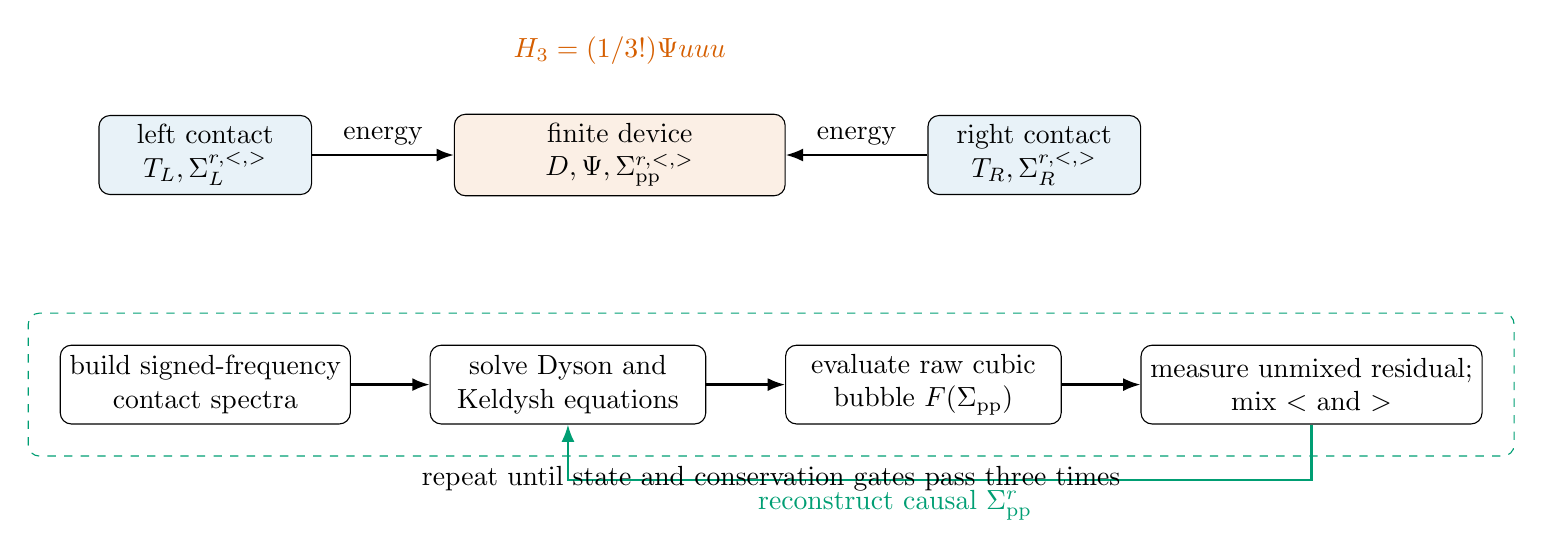
\begin{tikzpicture}[
  box/.style={draw,rounded corners,align=center,minimum height=10mm,
              minimum width=27mm,fill=white},
  contact/.style={box,fill=negfblue!9},
  device/.style={box,fill=negforange!10,minimum width=42mm},
  iterationbox/.style={box,minimum width=35mm},
  arrow/.style={-{Latex[length=2.2mm]},thick},
  loop/.style={-{Latex[length=2.2mm]},thick,negfgreen}
]
\node[contact] (left) {left contact\\\(T_L,\Sigma_L^{r,<,>}\)};
\node[device,right=18mm of left] (dev) {finite device\\\(D,\Psi,\Sigma_\pp^{r,<,>}\)};
\node[contact,right=18mm of dev] (right) {right contact\\\(T_R,\Sigma_R^{r,<,>}\)};
\draw[arrow] (left) -- node[above]{energy} (dev);
\draw[arrow] (right) -- node[above]{energy} (dev);
\node[above=5mm of dev,negforange] {\(H_3=(1/3!)\Psi uuu\)};

\node[iterationbox,below=19mm of left] (contacts) {build signed-frequency\\contact spectra};
\node[iterationbox,right=10mm of contacts] (solve) {solve Dyson and\\Keldysh equations};
\node[iterationbox,right=10mm of solve] (bubble) {evaluate raw cubic\\bubble \(F(\Sigma_\pp)\)};
\node[iterationbox,right=10mm of bubble] (mix) {measure unmixed residual;\\mix \(<\) and \(>\)};
\draw[arrow] (contacts) -- (solve);
\draw[arrow] (solve) -- (bubble);
\draw[arrow] (bubble) -- (mix);
\draw[loop] (mix.south) -- ++(0,-7mm) -|
node[pos=0.28,below]{reconstruct causal \(\Sigma_\pp^r\)}
(solve.south);
\node[fit=(contacts)(solve)(bubble)(mix),draw=negfgreen,dashed,
      rounded corners,inner sep=4mm,label=below:{repeat until state and
      conservation gates pass three times}] {};
\end{tikzpicture}}
\caption{\textbf{Production device partition and SCBA loop.}
The interaction is confined to the finite device; contacts are harmonic.
The fixed-point residual is evaluated before mixing. Lesser and greater
self-energies are mixed together and the retarded part is reconstructed
afterward. A nonzero device regulator is absent from this certified branch.}
\label{fig:formalism}
\end{figure}

\section{Frequency grid, SCBA iteration, and diagnostics}

\subsection{Signed grid and convolution}

The dense reference solver uses the odd signed grid
\begin{equation}
\omega_n=n\Delta\omega,\qquad n=-N,\ldots,N,
\end{equation}
with equal rectangle weight \(\Delta\omega/(2\pi)\). The convolution in
\cref{eq:bubble} uses integer index arithmetic and zero extension outside
the cutoff. Circular wraparound is forbidden. Initial cubic calculations use
a cutoff of at least three times the harmonic band edge and then refine it.

\subsection{SCBA algorithm}

The implemented iteration is:
\begin{enumerate}
  \item build \(\Sigma_{L/R}^{r,<,>}\) on the signed grid;
  \item initialize \(\Sigma_\pp^{<,>}=0\), or load a continuation state;
  \item reconstruct \(\Sigma_\pp^r\) with \cref{eq:hilbert};
  \item solve \cref{eq:dyson,eq:keldysh};
  \item evaluate the raw bubble \(F(\Sigma_\pp)\);
  \item measure the \emph{unmixed} residual \(F(\Sigma_\pp)-\Sigma_\pp\);
  \item mix the lesser and greater components together and reconstruct the
  retarded component;
  \item halve the initial mixing \(0.2\) after three successive residual
  increases, down to a floor of \(0.01\);
  \item require state, identity, and conservation gates for three consecutive
  iterations.
\end{enumerate}
At 200 iterations, the production API raises an exception carrying the last
complete partial result. One-shot Born has fixed semantics: construct
contact-only \(G_0\), evaluate one bubble, and perform one updated
Dyson/Keldysh solve. It is diagnostic and is not expected to conserve current.

\subsection{Required identities}

The automated checks include
\begin{align}
G^a&=G^{r\dagger},&
G^>-G^<&=G^r-G^a,\\
G^{</>\dagger}&=-G^{</>},&
[G^>(\omega)]^T&=G^<(-\omega),\\
G^r(-\omega)&=G^r(\omega)^*,&
\omega^2G^r&\rightarrow I .
\end{align}
They also test signed spectral passivity, the first spectral moment,
equilibrium KMS/FDT identities, \cref{eq:conservation}, independent fixed-point
recomputation, cutoff tails, and a bounded converged
serial/direct--threaded/direct--FFT/FFT oracle. For onsite or strictly
intralayer bare cubic vertices, the raw harmonic bond-current field is a
spatial gate only when the self-consistent interaction self-energy is block
local, \(r_{\rm nl}\leq10^{-12}\). Full nonlocal SCBA can generate off-layer
\(\Sigma_{pp}\) even from an intralayer bare vertex; in that case raw bond
currents are diagnostic, while projected-EOM-corrected cut currents and the
continuity residual are the spatial gates. The projected EOM and
layer-collision sums must each recover the global \(P_{pp}\). A cross-cut
FPU-\(\alpha\) vertex still requires a separately derived Hamiltonian
interaction-current operator.

\section{Named approximation levels}
\label{sec:approximations}

\begin{table}[t]
\centering
\caption{\textbf{Approximation hierarchy.} Historical methods are isolated
from the production Guo-convention solver. ``Validated'' below refers only
to the stated toy evidence, not to real-material FC3 calculations.}
\label{tab:approximations}
\small
\begin{tabularx}{\textwidth}{@{}p{29mm}p{28mm}p{29mm}p{27mm}X@{}}
\toprule
Method & Dynamic term & Propagators & Static term & Status \\
\midrule
Harmonic NEGF & none & contact-dressed \(G_0\) & none &
validated harmonic path \\
Guo one-shot Born & production bubble, once & \(G_0G_0\) & none &
fast screening and SCBA initialization; not generally conserving \\
Guo SCBA & production bubble, iterated & dressed \(GG\) & none &
production conductance method; dense toy gate certified \\
Wang \(O(T^2)\) & historical contour bubble & \(G_0G_0\) &
fixed \(G_0\) tadpole & source-limited historical regression \\
Wang selective MF & iterated contour bubble & dressed \(GG\) bubble &
fixed \(G_0\) tadpole & historical only; not a production oracle \\
Wang \(O(T^4)\) & \(O(T^2)\) plus six diagrams & perturbative \(G_0\) &
paper diagrams & unimplemented, nonblocking historical extension \\
Mingo Eq.~(27) & \((\pi/9)\Sigma_{\rm Guo}\) & intended dressed \(GG\) &
none & convention map audited; reproduction unresolved \\
\bottomrule
\end{tabularx}
\end{table}

\subsection{Convention mappings}

The same phrase ``third-order force constant'' denotes different Hamiltonian
coefficients in the literature. Under consistent mass normalization,
\begin{align}
\text{NEGFPy/Guo:}\quad&
H_3=\frac{1}{3!}\Psi_{ijk}u_i u_j u_k,\\
\text{Wang:}\quad&
H_n=\frac{1}{3}T_{ijk}u_i u_j u_k,
\qquad \Psi_{ijk}=2T_{ijk},\\
\text{Mingo:}\quad&
H_3=V^{(3)}_{ijk}\phi_i\phi_j\phi_k,
\qquad \Psi_{ijk}=6\widetilde V^{(3)}_{ijk}.
\end{align}
Here \(O(T^n)\) denotes order in Wang's cubic tensor \(T_{ijk}\), not order
in temperature.
For Mingo's molecular model,
\begin{equation}
V''=2k_m,\qquad V'''=\beta V'',
\end{equation}
and the audited printed-kernel relation is
\begin{equation}
\Sigma_{\text{Mingo Eq.~(27)}}^{</>}=
\frac{\pi}{9}\Sigma_{\text{Guo}}^{</>}.
\label{eq:mingo-map}
\end{equation}
The Wang dynamic bubble maps to the production bubble after \(\Psi=2T\), but
the fixed tadpole, contour retarded construction, and selective dressing make
the complete historical approximations different.

\begin{figure}[t]
\centering
\resizebox{0.98\textwidth}{!}{
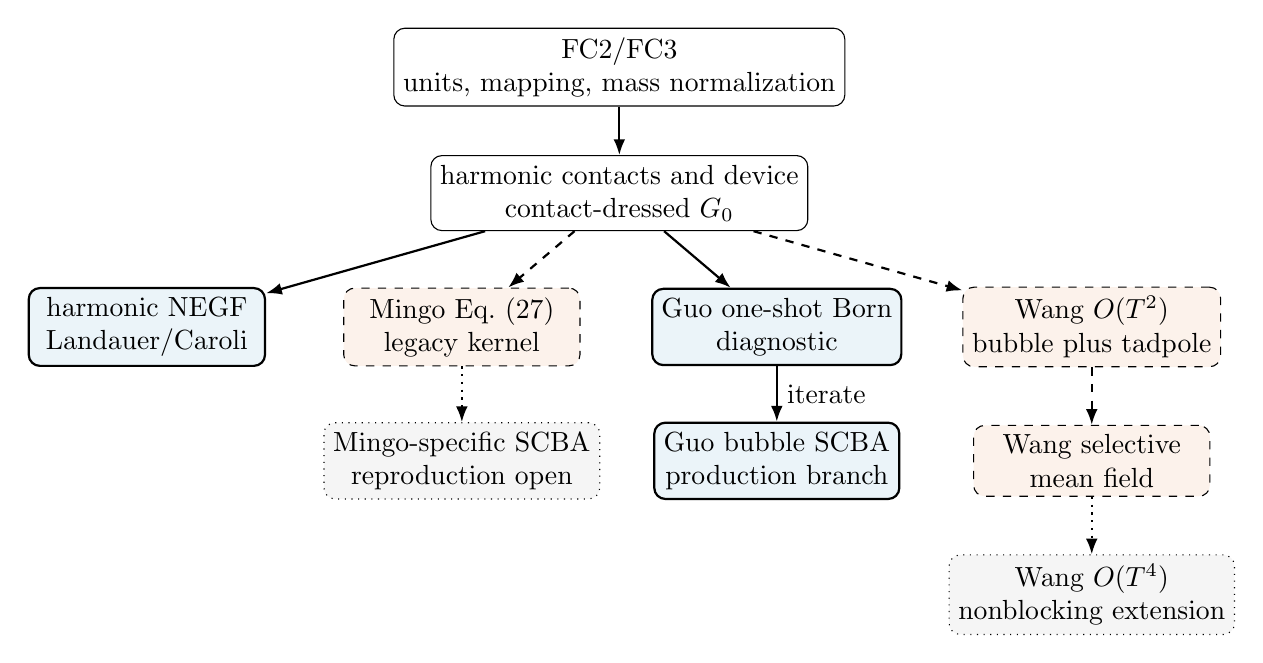
\begin{tikzpicture}[
  box/.style={draw,rounded corners,align=center,minimum width=30mm,
              minimum height=9mm},
  prod/.style={box,thick,fill=negfblue!8},
  hist/.style={box,dashed,fill=negforange!8},
  open/.style={box,dotted,fill=black!4},
  arr/.style={-{Latex[length=2mm]},thick}
]
\node[box] (ifc) at (0,1.6)
  {FC2/FC3\\units, mapping, mass normalization};
\node[box] (g0) at (0,0)
  {harmonic contacts and device\\contact-dressed \(G_0\)};

\node[prod] (harm) at (-6.0,-1.7)
  {harmonic NEGF\\Landauer/Caroli};
\node[hist] (mingok) at (-2.0,-1.7)
  {Mingo Eq.~(27)\\legacy kernel};
\node[open] (mingos) at (-2.0,-3.4)
  {Mingo-specific SCBA\\reproduction open};

\node[prod] (born) at (2.0,-1.7)
  {Guo one-shot Born\\diagnostic};
\node[prod] (scba) at (2.0,-3.4)
  {Guo bubble SCBA\\production branch};

\node[hist] (wang2) at (6.0,-1.7)
  {Wang \(O(T^2)\)\\bubble plus tadpole};
\node[hist] (wangmf) at (6.0,-3.4)
  {Wang selective\\mean field};
\node[open] (wang4) at (6.0,-5.1)
  {Wang \(O(T^4)\)\\nonblocking extension};

\draw[arr] (ifc) -- (g0);
\draw[arr] (g0) -- (harm);
\draw[arr,dashed] (g0) -- (mingok);
\draw[arr,dotted] (mingok) -- (mingos);
\draw[arr] (g0) -- (born);
\draw[arr] (born) -- node[right]{iterate} (scba);
\draw[arr,dashed] (g0) -- (wang2);
\draw[arr,dashed] (wang2) -- (wangmf);
\draw[arr,dotted] (wangmf) -- (wang4);
\end{tikzpicture}}
\caption{\textbf{Implemented and open approximation branches.}
Solid blue boxes are production operations, dashed orange boxes are isolated
historical validation methods, and dotted boxes are unimplemented or
scientifically unresolved. A curve from one branch is never silently used as
an oracle for another.}
\label{fig:hierarchy}
\end{figure}

\subsection{Lead and device regulators}

\begin{table}[ht]
\centering
\caption{Regulator policy.}
\begin{tabular}{@{}lll@{}}
\toprule
Quantity & Production policy & Interpretation \\
\midrule
\(\eta_{\rm lead}\) & positive; independently refined &
surface-Green-function regulator \\
\(\eta_{\rm device}\) & exactly zero &
no unaccounted dissipative bath \\
finite device damping & explicit \(\Sigma^{r,<,>}\) &
physical auxiliary reservoir \\
\bottomrule
\end{tabular}
\end{table}

Historical Wang calculations use finite \(\eta_{\rm device}\) only to
near-reproduce the archived calculation and are always noncertifying. The
production campaign changes \(\eta_{\rm lead}\) independently. Because that
change modifies the contact resolvent, its pointwise fields are descriptive,
not a fixed-point route-equality gate; transport current, pole observables,
cutoff tails, and per-run conservation remain certification quantities.
Acoustic leads and real materials are outside the present evidence.
\section{Certified production toy-gate evidence}
\label{sec:production-evidence}

\subsection{Fail-closed evidence contract}

This document accepts exactly the imported evidence and rendered figure
trees named in the required, generated \code{release_config.tex}. The
importer checks the raw
report and nested body digests, exact Git commit, source-tree hash,
environment-lock hash, fetched-manifest hash, complete run topology, and the
static and runtime contracts. The figure renderer independently binds its
inputs to the import receipt. Compilation then stops before producing a
manuscript unless the generated release summary declares
\code{ToyGateReleaseCertified=true}.

The four top-level results imported from the strict report are:
\begin{center}
\begin{tabular}{@{}ll@{}}
\toprule
Gate & Imported value \\
\midrule
Independent open-system oracle & \texttt{\ToyGateOraclePassed} \\
Nine-DOF multidimensional SCBA & \texttt{\ToyGateMultidimensionalPassed} \\
Static configuration contract & \texttt{\ToyGateStaticConfigurationPassed} \\
Runtime evidence contract & \texttt{\ToyGateRuntimeEvidencePassed} \\
\bottomrule
\end{tabular}
\end{center}
The top-level declaration is an aggregate, not a substitute for the
run-level evidence below. All numerical entries in the following tables are
generated from the same validated JSON document.

\begin{table}[t]
\centering
\caption{\textbf{Locked acceptance contract used by the strict report.}
Absolute tolerances remain active wherever a relative quantity is near zero.}
\label{tab:acceptance-contract}
\small
\begin{tabularx}{\textwidth}{@{}p{39mm}p{54mm}X@{}}
\toprule
Gate family & Threshold & Scope \\
\midrule
Open on-shell oracle agreement & \(5\times10^{-3}\) relative & linewidth and dynamic shift \\
Zero/Born and direct/continuation & rtol \(10^{-8}\), atol \(10^{-12}\) & six fields plus \(J_{\rm tr}\) \\
Bounded backend oracle & rtol \(10^{-10}\), atol \(10^{-12}\) & six fields plus full current/conservation vector \\
Directional numerical refinement & \(5\times10^{-3}\) & \(J_{\rm tr}\), selected FWHM, and shift \\
Outer self-energy tail & \(10^{-6}\) & every critical refinement \\
Weak coupling & \(\Gamma/\Omega<0.1\), \(|\Delta\Omega|/\Omega<0.1\) & released open and nine-DOF points \\
KMS/FDT/Keldysh & \(10^{-8}\) & applicable equilibrium identities \\
Conservation & \(\max[10^{-10}J_0,10^{-5}\max(|J_L|,|J_R|)]\) & contact balance and \(P_{pp}\), independently \\
\bottomrule
\end{tabularx}
\end{table}

\begin{table}[p]
\centering
\caption{\textbf{Seven-point harmonic same-grid preflight.} The base point
and all six preregistered numerical directions are mandatory archived
evidence before any SCBA result is accepted. Only the four declared
directional comparisons are certification critical; the other directions
remain visible diagnostics.}
\label{tab:harmonic-preflight}
\scriptsize
\resizebox{\textwidth}{!}{%
\begin{tabular}{@{}llrrrrrrll@{}}
\toprule
Point & role & $\Delta\omega$ & cutoff & $\eta_{\rm lead}$ & mixing &
$J_{\rm tr}/J_0$ & moment residual & point & comparison \\
\midrule
\TableRowsInput{\ProductionStagingDir/tex/harmonic_preflight_rows.tex}
\bottomrule
\end{tabular}}
\end{table}

\subsection{Independent open-system oracle and one-shot Born}
\label{sec:production-open}

The continuum fixture contains three unit-mass modes with centers
\begin{equation}
  (\Omega_p,\Omega_1,\Omega_2)=(1.5,0.9,0.6),
  \qquad \Omega_p=\Omega_1+\Omega_2,
\end{equation}
diagonal harmonic leads, lead coupling \(0.1\), and the local interaction
\(H_3=g u_pu_1u_2\). The independent oracle evaluates analytic scalar
surface spectra, explicit Bose emission and absorption channels, adaptive
continuum convolution, and principal-value quadrature. It does not call the
production cubic contraction or retarded-reconstruction functions. The
production comparison uses the fixed one-shot Born semantics and the
unmodified \(i\hbar/2\) coefficient in \cref{eq:bubble}.

The oracle is eta-free. The production base matrix is
\(T\in\{0,0.7\}\), \(g\in\{-0.02,-0.01,0,0.01,0.02\}\), with
\(\Delta\omega=7.0\times10^{-5}\), \(n_{\rm positive}=71571\)
(143143 signed points and \(\omega_{\rm cut}=5.00997\)), and
\(\eta_{\rm lead}=4.5\times10^{-5}\). Three additional outcomes at
\((T,g)=(0.7,0.02)\) independently halve the spacing, raise the cutoff to
6, or halve \(\eta_{\rm lead}\), giving thirteen archived outcomes in total.

The compared quantities are weak-coupling on-shell estimates, not a
complex-pole solve or fitted spectral peak:
\begin{equation}
  \Gamma_p=-\frac{\operatorname{Im}[\Sigma^r_{\pp}(\Omega_p)]_{pp}}
                   {\Omega_p},
  \qquad
  \Delta\Omega_p=
  \frac{\operatorname{Re}[\Sigma^r_{\pp}(\Omega_p)]_{pp}}
       {2\Omega_p}.
\end{equation}
Here \(\Gamma_p\) is the spectral FWHM (equivalently the population-decay
rate in this convention), so the spectral HWHM is \(\Gamma_p/2\).
\(\Delta\Omega_p\) is the dynamic cubic-bubble shift only; the excluded
cubic tadpole/static shift is not included.

The thirteen signed-coupling outcomes in \cref{tab:open-production} include
zero and finite temperature, \(g\leftrightarrow-g\), coupling scaling,
spontaneous decay, and numerical refinements. ``Maximum oracle-agreement gate
ratio'' is the larger of the production-versus-oracle linewidth and shift
error divided by its allowed error; a passing value is at most one. Near-zero
observables use the preregistered absolute tolerance rather than an unstable
relative error.

\begin{table}[p]
\centering
\caption{\textbf{Complete open-system production matrix.} Values are in
reduced solver units. Every row is generated from the immutable strict
report; no value is copied from an earlier exploratory benchmark.}
\label{tab:open-production}
\scriptsize
\begin{tabular}{@{}lrrrrrl@{}}
\toprule
Alias & \(T\) & \(g\) & \(\Gamma_p\) & \(\Delta\Omega_p\) &
max. oracle ratio & oracle agreement \\
\midrule
\TableRowsInput{\ProductionStagingDir/tex/open_run_rows.tex}
\bottomrule
\end{tabular}
\end{table}

\begin{figure}[p]
\centering
\includegraphics[width=\textwidth]{\ProductionFigureDir/figure_open_oracle_born.pdf}
\caption{\textbf{Independent oracle and production one-shot Born gate.}
(a) Parent linewidth and (b) on-shell shift across the signed-coupling matrix.
(c) Production-versus-oracle parity for the on-shell linewidth and shift.
(d) Sign invariance, \(g^2\) scaling, spontaneous-decay, and refinement ratios normalized by their
predeclared limits. The vector PDF is accompanied by a 450-dpi RGB PNG; both
are generated only from the receipt-bound staging data.}
\label{fig:production-open}
\end{figure}

This gate validates the cubic self-energy magnitude and on-shell dynamic
shift in
the weak-coupling open-system fixture. One-shot Born remains a diagnostic:
because it does not solve the nonlinear conserving fixed point, it is not a
standalone interacting-conductance certification method.

\subsection{Nine-degree-of-freedom conserving SCBA campaign}
\label{sec:production-scba}

The multidimensional device contains three layers and three polarizations per
layer. Each layer has the local permutation-symmetric vertex
\(g u_xu_yu_z\). The preregistered graph contains the zero-coupling and
interacting equilibrium path, the finite-bias continuation path, independent
spacing, cutoff, lead-\(\eta\), and mixing changes, zero and Born endpoint
starts, and a deterministic backend comparison. The thirteen archived
outcomes comprise eleven certification-required runs and two deliberately
diagnostic runs. A diagnostic failure cannot be silently discarded, and a
diagnostic run cannot replace a required one.

The physical ladder is \(g\in\{0,0.025,0.05\}\) at mean temperature
0.7 with \(\Delta T\in\{0,0.1,0.2\}\). The base controls are
\(\Delta\omega=0.00078125\), cutoff 5,
\(\eta_{\rm lead}=0.0015625\), and mixing 0.2. Independently archived
controls use spacing \(0.0015625\) and \(0.000390625\), cutoff 6,
lead eta \(0.003125\) and \(0.00078125\), and mixing 0.1. Every full-grid
SCBA outcome uses exact zero-padded FFT convolution, the FFT implementation
of the same finite-grid principal-value sum, and analytic diagonal contacts.
Serial/direct, threaded/direct, and FFT/FFT equality is established only by
the separate bounded converged oracle.

\begin{table}[p]
\centering
\caption{\textbf{All thirteen dense SCBA outcomes.} Current is reported in
\(J_0=\hbar\omega_0^2\). The row-level certification flag includes the
fixed-point, identity, conservation, and provenance checks applicable to that
outcome. The nine-DOF weak-coupling requirement is a separate campaign-level
gate and is reported separately below.}
\label{tab:scba-outcomes}
\scriptsize
\resizebox{\textwidth}{!}{%
\begin{tabular}{@{}llrrlrrl@{}}
\toprule
Alias & role & \(g\) & \(\Delta T\) & initialization & iterations &
\(J_L/J_0\) & row certified \\
\midrule
\TableRowsInput{\ProductionStagingDir/tex/scba_outcome_rows.tex}
\bottomrule
\end{tabular}}
\end{table}

\begin{table}[t]
\centering
\caption{\textbf{Weak-coupling scope of the released toy points.}
The two summaries are derived independently from all thirteen open-system
records and all thirteen nine-DOF outcomes. Ratios must be strictly below
the locked limit; they are not fit parameters.}
\label{tab:weak-coupling-production}
\small
\begin{tabular}{@{}lrrrrl@{}}
\toprule
Fixture & coverage & max. $\Gamma/\Omega$ &
max. $|\Delta\Omega|/\Omega$ & limit & passed \\
\midrule
Open three-mode & \ToyGateWeakCouplingCoverage &
\ToyGateWeakCouplingMaxLinewidthRatio &
\ToyGateWeakCouplingMaxShiftRatio & \ToyGateWeakCouplingLimit &
\texttt{\ToyGateWeakCouplingPassed} \\
Nine-DOF SCBA & \ToyGateMultidimensionalWeakCouplingCoverage &
\ToyGateMultidimensionalWeakCouplingMaxLinewidthRatio &
\ToyGateMultidimensionalWeakCouplingMaxShiftRatio &
\ToyGateMultidimensionalWeakCouplingLimit &
\texttt{\ToyGateMultidimensionalWeakCouplingPassed} \\
\bottomrule
\end{tabular}
\end{table}

\begin{figure}[p]
\centering
\includegraphics[width=\textwidth]{\ProductionFigureDir/figure_scba_validation.pdf}
\caption{\textbf{Conserving nine-DOF production campaign.}
(a) The preregistered coupling-and-bias path. (b) Endpoint fixed-point
convergence. (c) Contact balance, cubic collision power, and spatial
continuity checks normalized by their gates. (d) Independent spacing,
cutoff, lead-\(\eta\), and mixing refinements. Panel (a) plots the archived
left-contact current \(J_L\) along the L-shaped path; cross-route and
refinement comparisons in panel (d) use \(J_{\rm tr}=(J_L-J_R)/2\).
Collision power is never folded into that comparison vector.}
\label{fig:production-scba}
\end{figure}

The SCBA stopping rule uses the \emph{unmixed} map residual and requires
three consecutive passes. Zero/Born and direct/continuation routes compare
all six fields \(G^{r,<,>}\) and \(\Sigma_{\pp}^{r,<,>}\), together
with \(J_{\rm tr}=(J_L-J_R)/2\), at
\(\mathrm{rtol}=10^{-8}\), \(\mathrm{atol}=10^{-12}\). The bounded
backend oracle compares the same six fields and the full current/conservation
vector at \(\mathrm{rtol}=10^{-10}\),
\(\mathrm{atol}=10^{-12}\). All four directional refinements gate
\(J_{\rm tr}\), the selected FWHM and shift at \(5\times10^{-3}\), and
the outer interaction-self-energy tail at \(10^{-6}\). Lead-eta fields are
descriptive because eta changes the contact resolvent; spacing and cutoff
have no pointwise field gate because their grids differ. Mixing changes only
the route and therefore also recovers all six fields at the \(10^{-8}\)
route tolerance.

\begin{table}[p]
\centering
\caption{\textbf{Exact eight-comparison matrix.} ``Field gate ratio'' is
shown only when pointwise field comparison is physically and numerically
applicable; a dash is intentional, not missing evidence. Criticality and
pass/fail are imported from the strict report.}
\label{tab:comparisons}
\scriptsize
\begin{tabularx}{\textwidth}{@{}>{\raggedright\arraybackslash}p{34mm}>{\raggedright\arraybackslash}p{24mm}Xrll@{}}
\toprule
Name & kind & endpoints & max. field gate ratio & critical & passed \\
\midrule
\TableRowsInput{\ProductionStagingDir/tex/comparison_rows.tex}
\bottomrule
\end{tabularx}
\end{table}

\subsection{Conservation and scoped passivity}
\label{sec:production-diagnostics}

For conserving SCBA, the contact imbalance and internal collision power must
vanish independently as in \cref{eq:conservation}. The allowed scale is
\(\max[10^{-10}J_0,10^{-5}\max(|J_L|,|J_R|)]\). Although the cubic vertices
are intralayer, the dressed bubble can generate a nonlocal
\(\Sigma_{pp}\). The strict report therefore applies the raw harmonic
bond-current gate only in the block-local case and otherwise checks the
projected-EOM-corrected cut current and continuity residual. The projected
EOM and layer-collision sums must each recover the global \(P_{pp}\), in
addition to the two integral identities tabulated here.

\begin{table}[t]
\centering
\caption{\textbf{Independent equilibrium and nonequilibrium conservation
checks.} Ratios are absolute residuals divided by the allowed error.}
\label{tab:conservation-production}
\small
\begin{tabular}{@{}llrrrl@{}}
\toprule
Check & alias & \(J_L/J_0\) & contact ratio & collision ratio & passed \\
\midrule
\TableRowsInput{\ProductionStagingDir/tex/conservation_rows.tex}
\bottomrule
\end{tabular}
\end{table}

Lesser/greater correlation positivity of \(iC^{</>}\) is tested for every
stored Green, contact, interaction, and total spectrum in every state.
Retarded spectral passivity has a narrower contract: harmonic-contact
passivity is gated in every run, whereas Green-function, total-self-energy,
and interaction-self-energy retarded passivity is gated only at global
equilibrium or when the cubic interaction is zero. Their interacting
nonequilibrium values are archived as descriptive diagnostics and are never
clipped or projected. Reference~\cite{uhrig2019} is cited only for the
general need for an occupation-ordering hypothesis, not as a theorem about
this transport steady state.

\begin{table}[p]
\centering
\caption{\textbf{Scoped Green/total/interaction retarded-passivity
diagnostics.} The first column after the alias states applicability for the
Green function; the remaining entries are violation metrics for \(G\),
\(\Sigma_{pp}\), and the total self-energy where applicable. Contact
passivity is an all-run gate but is not repeated in this table.}
\label{tab:passivity-production}
\scriptsize
\begin{tabular}{@{}llrrr@{}}
\toprule
Alias & \(G^r\) applicable & \(G\) violation & \(\Sigma_{pp}\) violation &
\(\Sigma_{\rm tot}\) violation \\
\midrule
\TableRowsInput{\ProductionStagingDir/tex/passivity_rows.tex}
\bottomrule
\end{tabular}
\end{table}

\begin{figure}[p]
\centering
\includegraphics[width=\textwidth]{\ProductionFigureDir/figure_passivity_backend_timing.pdf}
\caption{\textbf{Diagnostic scope, bounded backend oracle, and cost.}
(a) Retarded-passivity applicability and (b) lesser/greater correlation
positivity applicability are shown explicitly. (c) The bounded converged
serial/direct, threaded/direct, and FFT/FFT backend oracle; it does not claim
direct or threaded SCBA on every full production grid. (d) Wall times retain
all required and diagnostic outcomes. Hardware-dependent timing is evidence
about cost, not a relaxed physics gate.}
\label{fig:production-passivity}
\end{figure}

\begin{table}[p]
\centering
\caption{\textbf{Cost and accuracy tiers.} Counts and aggregate wall times
are imported measurements, whereas the asymptotic expressions state the
dense-algorithm scaling. The timings are not controlled speedups and do not
change the scientific role of any method.}
\label{tab:cost-accuracy}
\scriptsize
\begin{tabularx}{\textwidth}{@{}p{19mm}Xccp{34mm}rrX@{}}
\toprule
Method & accuracy role & SC & conserving & dense time & count & total (s) &
release use \\
\midrule
\TableRowsInput{\ProductionStagingDir/tex/cost_accuracy_rows.tex}
\bottomrule
\end{tabularx}
\end{table}

\subsection{Failed-attempt audit and correction of the eta policy}

An earlier immutable campaign at Git revision
\code{1c6be52} completed its run graph but remained noncertifying. The audit
found three contract errors: a transport comparison vector included the
near-zero internal collision power, pointwise fields were gated across a
lead-\(\eta\) change even though that change modifies the contact resolvent,
and runtime evidence was mislabeled as a static-configuration mismatch.
None of those failures was removed by fitting an interaction prefactor or by
retuning a numerical point.

Revision \code{820d40250fede330c246e59613c2ca2d1c8279de} froze the corrected
policy and produced the historical certified toy baseline: transport uses
\(J_{\rm tr}=(J_L-J_R)/2\), collision power and contact balance remain
independent conservation gates, and field equality is required only for
comparisons that represent the same operator and grid. All six refinement
points remain archived, including diagnostic directions. That revision is
historical evidence only; it is not substituted for the newly integrated
candidate named by \texttt{\ExpectedToyGateCommit}.

The first local launch of the historical revision, labeled
\code{attempt-001}, stopped at the provenance preflight before any SCBA
outcome. The explicit dependency lock had been created correctly, but the
committed editable package-install step had been omitted, so the installed
NEGFPy version was reported as unknown even though the Git revision, source
hash, and clean-tree checks were already correct. That failed attempt is
checksum sealed as noncertifying. The missing deployment step was restored
exactly as committed, and \code{attempt-002} used a fresh checkpoint
directory with unchanged physical and numerical controls. The current
candidate reruns the complete gate from its own clean source and environment;
none of the historical numerical rows is imported as current evidence.

\subsection{Task-level MPI correctness and remote scaling}
\label{sec:mpi-evidence}

MPI is an orchestration layer above the numerical solver. Rank zero
coordinates complete validation cases, workers execute one whole case at a
time, and MPI carries identifiers and terminal status only. No Green
function, self-energy, convolution, or floating-point reduction is split
across ranks. Consequently, changing rank count changes scheduling but not
the SCBA equations, finite-grid arithmetic, or convergence thresholds.

The preregistered \MPIRankLadder{} ladder uses five fresh, isolated
repetitions of the complete representative 28-task graph. This timing profile
is intentionally noncertifying; its role is to select resources. Every
repetition must complete with the same canonical physics digest before the
smallest rank count within 5\% of the fastest time is considered. The toy
campaign uses that candidate only if its speedup is at least \(2\times\);
otherwise it uses the serial/FFT fallback. The locked production campaign is
then rerun with the selected release count and must independently report
\code{release_certified=true}.

\begin{table}[t]
\centering
\caption{\textbf{Exact remote task-MPI selection and resource evidence.}
Values are generated from the verified scaling-selection and release-runner
artifacts; timing does not relax any physics gate.}
\label{tab:mpi-scaling}
\small
\begin{tabularx}{\textwidth}{@{}p{58mm}X@{}}
\toprule
Field & imported value \\
\midrule
Preregistered rank ladder & \MPIRankLadder \\
Fastest rank count & \MPIFastestRankCount \\
Smallest rank count within 5\% of fastest & \MPICandidateRankCount \\
One-rank / candidate wall time (s) &
\(\MPIBaselineWallSeconds / \MPICandidateWallSeconds\) \\
Candidate speedup & \(\MPICandidateSpeedup\times\) \\
Locked toy release execution &
\MPIReleaseMode{} on \MPIReleaseRankCount{} rank(s) \\
Selected silicon target-\(q\) rank count & \MPISiliconRankCount \\
Physical sockets & \MPISocketCount \\
Maximum aggregate predicted / live available RAM &
\MPIMaxMemoryFractionObserved \\
\bottomrule
\end{tabularx}
\end{table}

Each launch measures Linux \code{MemAvailable} immediately before execution
and refuses the aggregate per-rank dense estimate above 0.70 of that live
value. BLAS and OpenMP thread counts are one. Runtime affinity records must
map every rank to exactly one distinct physical core; the even multi-rank
launches are distributed equally across the recorded sockets. The generator
rejects incomplete ladders, oversubscription, unbalanced sockets, stale
memory policy, noncanonical JSON, altered identities, or a release runner
whose source, environment, topology, and selected count do not match.

The coordinator uses a collective terminal handshake so that both scientific
and infrastructure failures reach every rank before shutdown. If a worker
was interrupted after atomically publishing a case artifact but before
publishing its task receipt, restart adopts that orphan only after validating
its exact task, source, environment, configuration, and content hashes. A
focused interruption test resumes a genuinely partial two-rank campaign with
four ranks and requires the same canonical physics projection used for
rank-equality decisions. It does not claim byte equality of the full report,
whose timing and orchestration provenance necessarily change with rank count.
These failure-atomic shutdown, orphan-adoption, and changed-rank partial
restart tests validate scheduler semantics; they do not change a scientific
failure or retune its controls.

The exact digest anchors are printed one per line so no abbreviated provenance
is used:
\begin{center}
\begin{tabular}{@{}l@{}}
Scaling-profile physics: \\[-1mm]
\quad{\scriptsize\texttt{\MPIScalingPhysicsSHA}} \\[1mm]
Release-profile physics: \\[-1mm]
\quad{\scriptsize\texttt{\MPIReleasePhysicsSHA}} \\[1mm]
Scaling-selection file: \\[-1mm]
\quad{\scriptsize\texttt{\MPIScalingManifestSHA}} \\[1mm]
Release-runner file: \\[-1mm]
\quad{\scriptsize\texttt{\MPIRunnerManifestSHA}} \\[1mm]
MPI execution-manifest file: \\[-1mm]
\quad{\scriptsize\texttt{\MPIExecutionManifestSHA}} \\[1mm]
Current-attempt pointer / selected immutable publication: \\[-1mm]
\quad{\scriptsize\texttt{\CurrentAttemptSHA}} \\[-1mm]
\quad{\scriptsize\texttt{\AttemptPublicationSHA}} \\[1mm]
MPI release-launch intent file / canonical payload: \\[-1mm]
\quad{\scriptsize\texttt{\MPIReleaseLaunchIntentSHA}} \\[-1mm]
\quad{\scriptsize\texttt{\MPIReleaseLaunchIntentPayloadSHA}} \\[1mm]
MPI release-launch receipt file / canonical payload: \\[-1mm]
\quad{\scriptsize\texttt{\MPIReleaseLaunchSHA}} \\[-1mm]
\quad{\scriptsize\texttt{\MPIReleaseLaunchPayloadSHA}} \\[1mm]
Execution-source / environment-prefix / scrubbed-launch environment: \\[-1mm]
\quad{\scriptsize\texttt{\MPIExecutionSourceIdentitySHA}} \\[-1mm]
\quad{\scriptsize\texttt{\MPIEnvironmentPrefixManifestSHA}} \\[-1mm]
\quad{\scriptsize\texttt{\MPILaunchEnvironmentSHA}} \\[1mm]
Fetched artifact raw \code{SHA256SUMS}: \\[-1mm]
\quad{\scriptsize\texttt{\ArtifactSHA256SUMSRawSHA}} \\[1mm]
Local fetch receipt: \\[-1mm]
\quad{\scriptsize\texttt{\ArtifactFetchReceiptSHA}} \\[1mm]
Production staging raw \code{SHA256SUMS} / import receipt: \\[-1mm]
\quad{\scriptsize\texttt{\StagingSHA256SUMSRawSHA}} \\[-1mm]
\quad{\scriptsize\texttt{\StagingImportReceiptSHA}} \\[1mm]
Production figures raw \code{SHA256SUMS} / render receipt: \\[-1mm]
\quad{\scriptsize\texttt{\ProductionFiguresSHA256SUMSRawSHA}} \\[-1mm]
\quad{\scriptsize\texttt{\ProductionFiguresReceiptSHA}} \\[1mm]
Historical figures raw \code{SHA256SUMS} / render receipt: \\[-1mm]
\quad{\scriptsize\texttt{\HistoricalFiguresSHA256SUMSRawSHA}} \\[-1mm]
\quad{\scriptsize\texttt{\HistoricalFiguresReceiptSHA}} \\[1mm]
Strict report file / nested body: \\[-1mm]
\quad{\scriptsize\texttt{\ReleaseStrictReportFileSHA}} \\[-1mm]
\quad{\scriptsize\texttt{\ReleaseStrictReportBodySHA}}
\end{tabular}
\end{center}

\section{Relationship to Wang and Mingo}
\label{sec:historical-status}

\subsection{Wang: useful computational tier, not the production oracle}

Wang, Wang, and Zeng use a contour expansion containing a leading
\(O(T^2)\) bubble, a static tadpole contribution, six additional
\(O(T^4)\) diagrams, and a selective mean-field construction
\cite{wang2006}. Under the Hamiltonian conventions in
\cref{sec:approximations}, the dynamic \(O(T^2)\) bubble can be mapped to the
production vertex normalization, but the full approximation cannot: its
tadpole, finite regulator, contour reconstruction, and dressing policy are
different.

The implemented Wang \(O(T^2)\) path is therefore a source-limited
historical regression, not a production oracle. The APS/Grace source is a
vector EPS path, not raster digitization. Conditional on the explicitly
inferred onsite-unit convention, the independent harmonic calculation over
all 51 vector-path temperatures has RMS/max errors
\(0.000124/0.000277\;\mathrm{nW\,K^{-1}}\). The complete historical
\(O(T^2)\) bubble-plus-tadpole result differs from the interpolated path by
0.49\%, 0.27\%, and 0.30\% at 100, 300, and 500 K; selective mean field
differs by 0.28\% and 0.75\% at 300 and 400 K. These are useful
source-limited regressions, but not a same-input reproduction because the
onsite assignment and plotted-run settings are not uniquely fixed by the
recoverable source. Wang \(O(T^4)\) remains unimplemented and nonblocking.
None of these rows contributes to production certification.

\subsection{Mingo: unresolved without a fitted normalization}

Mingo's molecular-junction calculation uses a different cubic Hamiltonian
normalization and a paper-specific surface spectral measure
\cite{mingo2006}. The printed convention can be mapped algebraically to
\cref{eq:h3,eq:bubble}, but the recoverable source information does not
uniquely determine the surface normalization and \(V'''/6\) convention
needed for a same-input interacting reproduction. Using the normalized
Eq.~(47) surface measure, the eta-free harmonic calculation differs from all
18 vector-path Fig.~4 points by \(3.2301\;\mathrm{pW/K}\) RMS and
\(5.0423\;\mathrm{pW/K}\) maximum; it is therefore not a same-input
reproduction. A separately named half-weight sensitivity gives
\(0.1264\;\mathrm{pW/K}\) RMS and \(0.2295\;\mathrm{pW/K}\) maximum, but
that factor is neither normalized nor derived from the printed equations and
is noncertifying. No interacting Mingo SCBA/Fig.~8 curve has been computed.
The status remains \emph{historical reproduction unresolved}; no surface
weight, vertex multiplier, or diagram coefficient is fitted.

\begin{figure}[p]
\centering
\includegraphics[width=\textwidth]{\HistoricalFigureDir/historical_paper_benchmarks.pdf}
\caption{\textbf{Noncertifying historical paper comparisons.} Published
coordinates are figure-extracted vector paths, not author raw data. Wang
results are conditional on the explicitly inferred onsite convention. The
Mingo half-weight curve is a sensitivity only, not a normalized production
choice; no interacting Mingo Fig.~8 calculation is shown. This separate
checksum-bound figure lane is historical evidence and is not part of the
production toy-gate certification.}
\label{fig:historical-paper-comparisons}
\end{figure}

\section{Certified scope, exclusions, and next gate}

The certified result applies to complex128 dense toy problems with harmonic
reservoirs, zero device regulator, a cubic bubble, causal principal-value
retarded reconstruction, and conserving SCBA. It validates the numerical
and physical contract needed before FC3 mapping. It does not establish the
following:

\begin{itemize}
  \item cubic tadpole or static equilibrium shifts;
  \item quartic Hartree/loop renormalization, four-phonon scattering,
  thermal expansion, or anharmonic reservoirs;
  \item acoustic \(\omega\rightarrow0\) support, which requires the analytic
  \(n_B\Gamma\) limit rather than a finite generic \(n_B(0)\);
  \item an FPU-\(\alpha\) cross-cut interaction-current operator;
  \item local-diagonal truncation, B\"uttiker probes, LOA/Pad\'e, mixed
  precision, sparse FC3 schedules, or transverse-momentum SCBA;
  \item high-temperature stability of a globally unbounded cubic potential;
  \item restart from an interrupted SCBA iteration inside one case and
  long-term pinned-host performance-regression certification. Task-level
  partial-campaign restart under a changed rank count is covered separately in
  \cref{sec:mpi-evidence};
  \item any real-material conductance, matrix element, phase space, or
  linewidth.
\end{itemize}

The proper next gate is the
\href{https://github.com/phonopy/phono3py/tree/v4.4.0/example/Si-PBEsol}
{pinned phono3py v4.4.0 Si-PBEsol example}.

\noindent Pinned source revision:
\code{302ad205452ee36e57887b10bbf4a0289dd037bb}.

\noindent Full and compact
\code{fc3.hdf5} inputs must follow the
\href{https://phonopy.github.io/phono3py/input-output-files.html#fc3-hdf5}
{official FC3 and gamma definitions}. FC3 is read in
\(\mathrm{eV}/\text{\AA}^3\), with explicit provenance and conversion;
phono3py gamma is stored in ordinary THz and is converted to angular
frequency exactly once by \(2\pi\). On identical meshes and smearing,
sampled \(|V^{(3)}|^2\) must agree to relative error below \(10^{-8}\);
among nonzero modes, linewidth median error must be below 1\% and maximum
error below 5\%, with a separately stated absolute tolerance for acoustic
modes. Material-device SCBA remains blocked until that bulk oracle passes;
sparse quasi-one-dimensional and transverse-periodic solvers follow
afterward.

\section{Provenance and reproducibility}

\begin{table}[t]
\centering
\caption{\textbf{Immutable production provenance.} These rows are generated
from the receipt-bound strict report.}
\label{tab:provenance}
\scriptsize
\begin{tabularx}{\textwidth}{@{}p{38mm}X@{}}
\toprule
Field & value \\
\midrule
\TableRowsInput{\ProductionStagingDir/tex/provenance_rows.tex}
\bottomrule
\end{tabularx}
\end{table}

The report package is deliberately two-stage. First, the local campaign is
finalized into a checksum-sealed artifact tree (or, for a remote campaign,
fetched with checksum verification) and imported with caller-supplied trust
anchors for the Git commit, environment lock, transport/publication receipt,
and raw \code{SHA256SUMS} file. The CLI retains
\code{--expected-fetch-receipt-sha256} as a legacy argument name for either
transport-receipt type. The importer writes the configured staging tree
atomically. Second, the renderer is given the independently computed
import-receipt hash and writes the configured production-figure tree
atomically. The three production
figures are embedded-font vector PDFs with 450-dpi RGB PNG companions.

The source manuscript never falls back to the legacy \path{data/} or
\path{figures/} evidence for a production result. To reproduce the document,
run the importer and renderer with their required external trust anchors,
then execute
\begin{verbatim}
latexmk -pdf -halt-on-error -interaction=nonstopmode \
  -outdir=output/pdf report.tex
\end{verbatim}
If the staging summary is absent, malformed, or noncertifying, the build
raises a named \code{NEGFPy toy-gate report} error before the manuscript body
is processed. Receipt hashes and file contents are authenticated by the
finalizer, importer, and renderer workflow; LaTeX itself checks only the
presence and literal values of the generated release, component-gate, and
commit macros.

\clearpage
\begin{thebibliography}{9}

\bibitem{wang2006}
J.-S. Wang, J. Wang, and N. Zeng,
``Nonequilibrium Green's function approach to mesoscopic thermal transport,''
\emph{Physical Review B} \textbf{74}, 033408 (2006).
\href{https://doi.org/10.1103/PhysRevB.74.033408}
{doi:10.1103/PhysRevB.74.033408}.

\bibitem{mingo2006}
N. Mingo,
``Anharmonic phonon flow through molecular-sized junctions,''
\emph{Physical Review B} \textbf{74}, 125402 (2006).
\href{https://doi.org/10.1103/PhysRevB.74.125402}
{doi:10.1103/PhysRevB.74.125402}.

\bibitem{guo2020}
Y. Guo \emph{et al.},
``Quantum mechanical modeling of anharmonic phonon-phonon scattering in
nanostructures,''
\emph{Physical Review B} \textbf{102}, 195412 (2020).
\href{https://doi.org/10.1103/PhysRevB.102.195412}
{doi:10.1103/PhysRevB.102.195412}.

\bibitem{uhrig2019}
G. S. Uhrig, M. H. Kalthoff, and J. K. Freericks,
``Positivity of the spectral densities of retarded Floquet Green functions,''
\emph{Physical Review Letters} \textbf{122}, 130604 (2019).
\href{https://doi.org/10.1103/PhysRevLett.122.130604}
{doi:10.1103/PhysRevLett.122.130604}.

\end{thebibliography}

\end{document}
